\chapter{Bootstrap ve Rastgeleleştirme ile Benzetime Dayalı Çıkarım}
\label{ch:resampling}

\begin{hedefler}
Bu bölümün sonunda:
\begin{itemize}
  \item yeniden örnekleme dağılımı ile kuramsal örnekleme dağılımını ayırt edebilecek,
  \item bootstrap yöntemiyle standart hata ve yüzdelik güven aralığı hesaplayabilecek,
  \item rastgeleleştirme testiyle sıfır hipotezi dağılımı ve \pval-değeri oluşturabilecek,
  \item benzetim tekrar sayısı, örneklem hacmi, temsil ve değiştirilebilirlik koşullarını değerlendirebileceksiniz.
\end{itemize}
\end{hedefler}

\begin{prerequisitebox}
Örnekleme dağılımı, nokta tahmini, standart hata, güven aralığı, sıfır
hipotezi ve \pval-değeri kavramları bilinmelidir. Rastgele örnek seçme ve temel
Python dizileri hakkında giriş düzeyinde bilgi yararlıdır.
\end{prerequisitebox}

\begin{hazirlik}
Aynı veriyi 10.000 kez yeniden kullanmak neden örneklem hacmini 10.000 katına
çıkarmaz? Özgün veri belirsizliği ile benzetim hatasını ayırın.
\end{hazirlik}

Tahmin edici ve standart hata kavramları Bölüm~\ref{ch:point-estimation}'de,
güven aralığının hedefi Bölüm~\ref{ch:confidence-intervals}'de açıklanmıştır.
Bu bölüm aynı hedeflere benzetim yoluyla yaklaşır.

\section{Neden yeniden örnekleme?}

Klasik çıkarım yöntemleri çoğu zaman normal veya Student t dağılımı gibi
kuramsal sonuçlara dayanır. Yeniden örnekleme yöntemleri ise gözlenen veriyi
tekrar tekrar düzenleyerek tahminin değişkenliğini veya sıfır hipotezi altında
beklenen sonuçları benzetimle görünür kılar.

Bu bölümde iki farklı soru ele alınır:

\begin{itemize}
  \item \textbf{Bootstrap:} Aynı evrenden yeni örneklemler seçebilseydik
  tahminimiz ne kadar değişirdi?
  \item \textbf{Rastgeleleştirme testi:} Sıfır hipotezi doğru olsaydı grup
  etiketlerini yeniden dağıttığımızda gözlenen kadar uç bir fark ne sıklıkla
  oluşurdu?
\end{itemize}

İki yöntemde de çok sayıda tekrar vardır; ancak tekrarların nasıl üretildiği
ve hangi dağılımın hedeflendiği farklıdır. Bootstrap kuramı ve uygulamaları
için \citet{efron1993} ile \citet{davison1997}; rastgeleleştirme testleri için
\citet{good2005} temel kaynaklardır.

\begin{definitionbox}
\textbf{Bootstrap}, gözlenen birimlerden yerine koyarak yeniden örnekleyip
tahminin değişkenliğini inceler. \textbf{Rastgeleleştirme testi} ise sıfır
hipotezi altında değiştirilebilir etiket veya işaretleri yeniden düzenleyip
test istatistiğinin başvuru dağılımını kurar.
\end{definitionbox}

\section{Bootstrap mantığı}
\label{sec:bootstrap}

$x_1,\ldots,x_n$ gözlenen örneklem olsun. Parametrik olmayan bootstrap
işlemi şu adımları izler:

\begin{enumerate}
  \item Gözlenen $n$ birimden yerine koyarak yine $n$ birim seçilir.
  \item Seçilen bootstrap örnekleminde hedef istatistik hesaplanır.
  \item İlk iki adım $B$ kez yinelenir.
  \item Elde edilen $\hat\theta_1^*,\ldots,\hat\theta_B^*$ değerlerinin
  dağılımı incelenir.
\end{enumerate}


Yerine koyarak seçim nedeniyle bir gözlem aynı bootstrap örnekleminde birden
fazla kez görülebilir, başka bir gözlem hiç seçilmeyebilir. Bootstrap
örnekleminin hacmi özgün örneklem hacmiyle aynıdır. Tekrar sayısı $B$'yi
artırmak özgün veriye yeni bilgi eklemez; yalnız benzetimden gelen Monte Carlo
dalgalanmasını azaltır.

Bootstrap standart hatası, tekrar tahminlerinin örneklem standart sapmasıdır:
\[
\SE_{\mathrm{boot}}(\hat\theta)
=\sqrt{\frac{1}{B-1}
\sum_{b=1}^{B}(\hat\theta_b^*-\bar{\theta}^*)^2}.
\]

\section{Bootstrap güven aralığı}
\label{sec:bootstrap-ci}

Yüzdelik bootstrap aralığında tekrar tahminlerinin alt ve üst yüzdelikleri
kullanılır. Yüzde 95 aralık yaklaşık olarak
\[
[\hat\theta^*_{0{,}025};\hat\theta^*_{0{,}975}]
\]
biçimindedir. Örneğin 10.000 tekrarın sıralanmış değerlerinde yüzde 2,5 ve
yüzde 97,5 noktaları aralığın uçlarını verir.

Yüzdelik yöntem sezgiseldir; fakat güçlü yanlılık, belirgin çarpıklık, çok
küçük örneklem veya dağılım sınırlarına yakın parametrelerde iyi çalışmayabilir.
Yanlılık düzeltilmiş ve hızlandırılmış BCa aralığı ya da probleme özgü başka
yöntemler gerekebilir. Bootstrap otomatik olarak bütün güven aralığı
sorunlarını çözen tek bir yöntem değildir.

\section{Rastgeleleştirme testinin mantığı}
\label{sec:randomization-test}

İki grup ortalaması veya oranı arasındaki fark incelensin. Sıfır hipotezi
grup etiketlerinin sonuç bakımından değiştirilebilir olduğunu söylüyorsa,
etiketler sonuç değerleri sabit tutularak rastgele karıştırılabilir:

\begin{enumerate}
  \item Gözlenen fark $T_{\text{göz}}$ hesaplanır.
  \item Grup etiketleri, grup hacimleri korunarak karıştırılır.
  \item Karıştırılmış veride $T_b^*$ hesaplanır.
  \item İşlem $B$ kez tekrarlanarak sıfır hipotezi dağılımı oluşturulur.
  \item Gözlenen kadar veya daha uç tekrarların oranı \pval-değerini verir.
\end{enumerate}

Sonlu benzetimde sıfır \pval-değeri raporlamamak için iki yönlü yaklaşık değer
\[
p_{\mathrm{rand}}
=\frac{1+\sum_{b=1}^{B}
\Ind{|T_b^*|\geq|T_{\text{göz}}|}}{B+1}
\]
biçiminde hesaplanabilir. Tek yönlü testte mutlak değer yerine önceden
belirlenen yön kullanılır.

Eşleştirilmiş veride bağımsız grup etiketleri karıştırılmaz. Sıfır değişim
hipotezi altında her çiftin fark işareti rastgele çevrilebilir. Yeniden
örnekleme şeması her zaman araştırma tasarımını korumalıdır.

\section{Bootstrap ile rastgeleleştirmenin karşılaştırılması}
\label{sec:resampling-comparison}

\begin{table}[H]
\centering
\small
\caption{İki yeniden örnekleme yönteminin temel farkları.}
\label{tab:resampling-comparison}
\begin{tabularx}{\textwidth}{@{}>{\raggedright\arraybackslash}p{0.22\textwidth}>{\raggedright\arraybackslash}X>{\raggedright\arraybackslash}X@{}}
\toprule
Özellik & Bootstrap & Rastgeleleştirme testi \\
\midrule
Temel hedef & Standart hata ve güven aralığı & Sıfır hipotezi ve \pval-değeri \\
Tekrar üretimi & Gözlemleri yerine koyarak seçme & Etiketleri veya fark işaretlerini karıştırma \\
Merkez & Genellikle gözlenen tahmin çevresi & Sıfır hipotezinin öngördüğü değer \\
Korunan yapı & Örneklem hacmi ve analiz birimi & Grup hacimleri ve araştırma tasarımı \\
Temel koşul & Örneklemin evreni yeterince temsil etmesi & Sıfır hipotezi altında değiştirilebilirlik \\
\bottomrule
\end{tabularx}
\end{table}

Tablo~\ref{tab:resampling-comparison}'deki ayrım önemlidir: bootstrap tahmin
belirsizliğini, rastgeleleştirme ise sıfır hipotezi altındaki uçluğu hedefler.

\section{Gerçek veride bootstrap uygulaması}

STAR98 verisindeki 303 okul bölgesi için ulusal matematik medyanının üzerinde
puan alan öğrenci oranlarının ortalaması yaklaşık 0,437'dir. Gözlenen okul
bölgelerinden 10.000 kez yerine koyarak 303 bölge seçilip her tekrarda ortalama
hesaplandığında bootstrap standart hatası yaklaşık 0,0106 bulunmuştur.
Yüzdelik yüzde 95 bootstrap aralığı
\[
[0{,}416;0{,}458]
\]
biçimindedir.

Analiz birimi okul bölgesidir. Bu nedenle aralık, tek tek öğrencilerin başarı
olasılığı için kurulmuş bir aralık değildir. Ayrıca veri bütün California
okul bölgelerinin olasılıklı örneği olarak seçilmediyse aralığın hangi hedef
evrene genellenebileceği ayrıca tartışılmalıdır.
STAR98 verisinin kaynağı ve okul bölgesi düzeyindeki yapısı için
\citet{gill2001} incelenebilir.

\section{Gerçek veride etiket permütasyonu}

Spector verisinde programa katılan 14 öğrencinin 8'inde, karşılaştırma
grubundaki 18 öğrencinin 3'ünde \texttt{GRADE=1} vardır. Burada kullanılan
statsmodels veri tanımı bunu not iyileşmesi olarak adlandırır
\citep{statsmodelsSpector}. Bu etiket başka bir kaynak sürümündeki sonuç
tanımıyla otomatik olarak eş tutulmaz. Gözlenen oran farkı
\[
\frac{8}{14}-\frac{3}{18}\approx0{,}405
\]
olur. Grup etiketleri 20.000 kez karıştırıldığında gözlenen mutlak fark kadar
veya daha uç 534 tekrar elde edilmiştir. Düzeltilmiş benzetim \pval-değeri
\[
p=\frac{534+1}{20\,000+1}\approx0{,}0267
\]
olarak bulunur. Bu benzetim sonucu aşağıdaki kodun tamamındaki işlem
sırasına aittir; aynı rastgele sayı üreteci önce bootstrap, sonra etiket
permütasyonu için kullanılır. Yalnız ikinci kısmı yeni bir üreteçle
çalıştırmak aynı uç tekrar sayısını vermek zorunda değildir.

Bu $p$ değeri, sıfır hipotezi altında grup etiketlerinin bu biçimde
değiştirilebilir olduğu varsayımıyla yorumlanır. Kodun etiketleri
karıştırabilmesi, özgün atamanın rastgele olduğunu göstermez. Atama
mekanizması burada doğrulanmadığından bu hesap, belgelenmiş bir deneyin
atama düzenini yeniden üreten test olarak değil, koşullu bir permütasyon
uygulaması olarak sunulur. Bu nedenle sonuç nedensel deney kanıtı olarak
değil, etiket değiştirilebilirliği koşuluna bağlı bir duyarlılık analizi
olarak yorumlanmalıdır.

\Needspace{8\baselineskip}
\subsection{Karşılaştırmalı görev: aynı öğrenciler, başka hedef}

\textbf{Analiz tanımı.} Yerel 32 kayıt korunur; grup büyüklükleri 14 ve
18'dir. Yanıt bu kez TUCE değil ikili GRADE göstergesidir. İstatistik,
program eksi karşılaştırma grubu oran farkıdır. Her tekrarda sonuçlar sabit
tutulur, 14 program etiketi 32 öğrenci arasında yeniden dağıtılır. Öğrenci
satırlarıyla yapılan bu işlem, sınıf düzeyindeki bir atamanın doğrulandığı
anlamına gelmez. Araştırma sınıfları birlikte atamışsa aynı permütasyon
düzeni gerekçesiz kullanılamaz.

\textbf{Görev ve teslim.} Aşağıdaki beş karşılaştırmayı gerekçelendirin.
\begin{enumerate}[label=\arabic*.]
\item TUCE için Welch testi ile GRADE için permütasyonda ne değişti?
Kayıt, yanıt, hedef büyüklük ve yöntem bakımından ayırın.
\item $8/14-3/18$ farkını yüzde puanla yazın. Bunun ``program başarıyı
yüzde 40,5 artırdı'' anlamına gelmediğini açıklayın.
\item Etiketler karıştırılırken nelerin sabit kaldığını belirtin.
Geçerli yorum için gereken varsayımı yazın.
\item Welch için 0,537, permütasyon için yaklaşık 0,0267 bulunması çelişki
midir? Anlamlı sonucu seçip diğerini gizleme önerisini değerlendirin.
\item ``20.000 karıştırma rastgele atamayı kanıtlar'' iddiasını düzeltin;
bulguyu sınırıyla raporlayın.
\end{enumerate}

\textbf{Gerekçeli kontrol yanıtları.}
(1) Kişiler aynıdır; TUCE ortalama farkı yerine GRADE oran farkı incelenir,
test yöntemi de değişir. (2) Fark yaklaşık 40,48 yüzde puandır; bu bir
göreli yüzde artışı ya da nedensel etki tahmini olarak sunulmaz.
(3) 32 sonuç, toplam 11 adet GRADE=1 ve 14/18 grup büyüklükleri korunur;
sonuçların hangi grup etiketine karşılık geldiği değişir. Seçilen sıfır
hipotezi altında bu etiket düzenlerinin değiştirilebilirliği gerekir.
(4) Sorular farklıdır; farklı kararlar çelişki değildir ve aynı veri iki
bağımsız tekrar oluşturmaz. (5) Tekrar sayısı bilgisayardaki benzetimi
tanımlar; saha atamasını belgelemez. Örnek rapor: ``GRADE=1 oranları
8/14 ve 3/18, fark 40,48 yüzde puandır. Belirtilen etiket permütasyonu
altında yaklaşık $p=0{,}0267$ elde edilmiştir; değiştirilebilirlik ve atama
dayanağı doğrulanmadığından bu değer tek başına program etkisi kanıtı
olarak sunulmamıştır.''

\textbf{Değerlendirme ölçütleri (10 puan).} Her madde 2 puandır:
(1) aynı kayıtları belirtme 1, değişen hedef/yöntem 1;
(2) yüzde puan hesabı 1, göreli artış ve nedensellikten ayırma 1;
(3) korunan büyüklükler 1, değiştirilebilirlik koşulu 1;
(4) soru farkı 1, sonuç seçmeme ve bağımsız tekrar saymama 1;
(5) benzetim--saha ataması ayrımı 1, sınırlı rapor 1.
Nedensel etki iddiası içeren son yanıt, doğru $p$ değeri yazsa bile rapor
puanını alamaz. Bu puanlama öğrenme etkisinin ölçülmüş olduğu anlamına gelmez.

\begin{figure}[H]
\centering
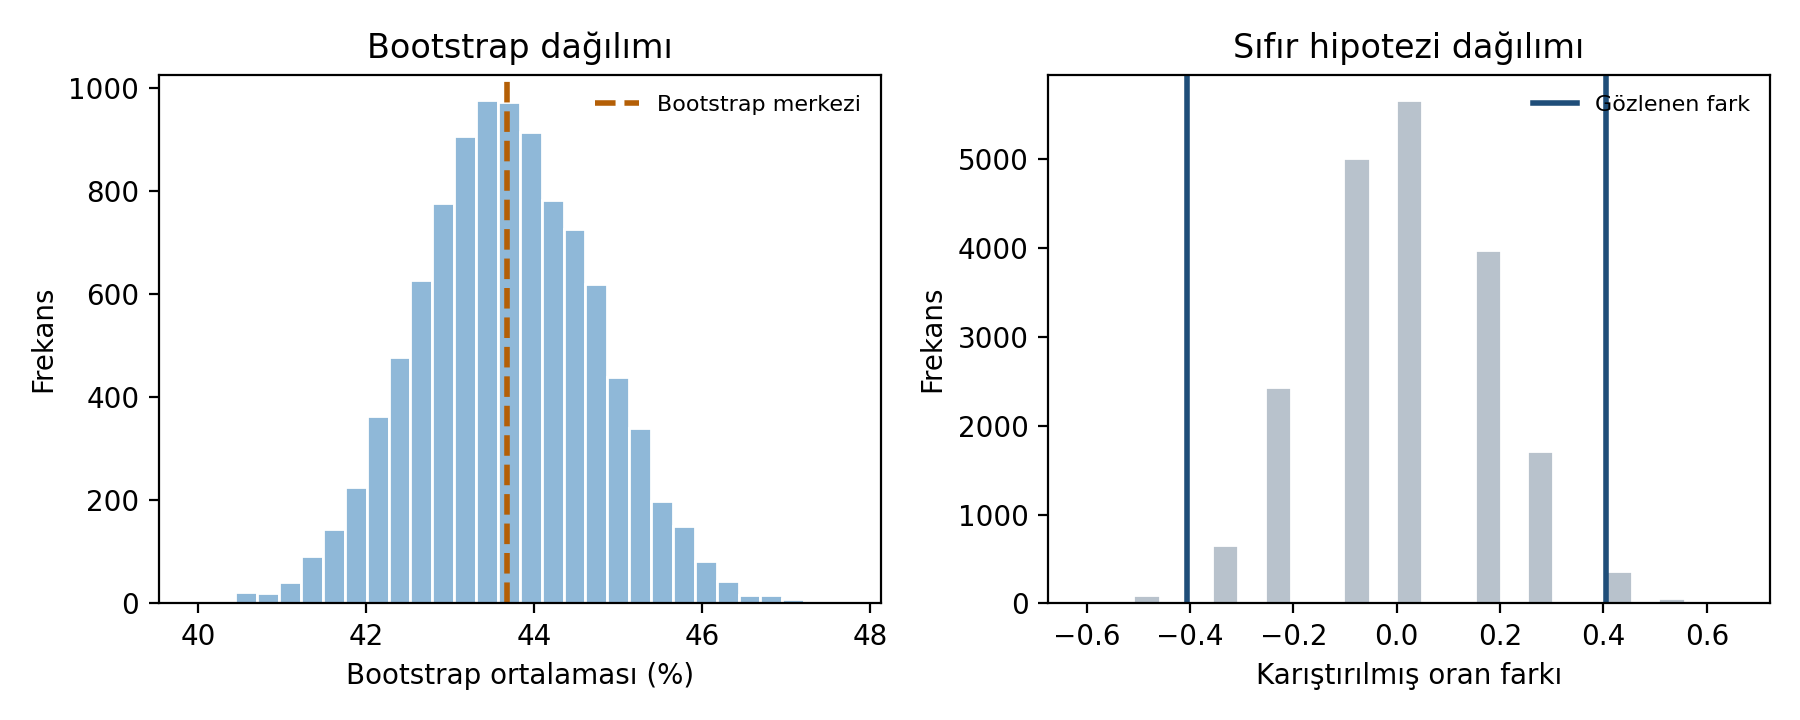
\includegraphics[width=\textwidth]{companion/outputs/figures/chapter09_resampling.png}
\caption{Gerçek veride bootstrap ve etiket permütasyonu dağılımları. Sol panel tahmin belirsizliğini, sağ panel belirtilen değiştirilebilirlik varsayımı altında oran farklarını gösterir; saha ataması bu grafikle doğrulanmaz.}
\label{fig:resampling-distributions}
\end{figure}

Şekil~\ref{fig:resampling-distributions}'de iki dağılımın farklı merkezleri,
bu farklı hedefleri görünür kılar.

\section{Yazılım uygulaması}

\begin{softwarebox}
\begin{lstlisting}
import numpy as np
import pandas as pd

rng = np.random.default_rng(2026)

# Bootstrap: okul bolgesi ortalamasi
star = pd.read_csv(
    "companion/data/clean/star98_districts.csv")
values = star["above_median_rate"].to_numpy()
B = 10000
boot = rng.choice(values, size=(B, len(values)),
                  replace=True).mean(axis=1)
print(boot.std(ddof=1), np.quantile(boot, [.025, .975]))

# Rastgelelestirme: iyilesme orani farki
data = pd.read_csv(
    "companion/data/clean/spector_program.csv")
labels = data["program_participation"].to_numpy()
outcome = data["grade_improved"].to_numpy()
observed = (outcome[labels == 1].mean()
            - outcome[labels == 0].mean())

randomized = np.empty(20000)
for b in range(len(randomized)):
    shuffled = rng.permutation(labels)
    randomized[b] = (outcome[shuffled == 1].mean()
                     - outcome[shuffled == 0].mean())

extreme = np.sum(np.abs(randomized) >= abs(observed))
p_value = (extreme + 1) / (len(randomized) + 1)
print(observed, p_value)
\end{lstlisting}
Tam uygulama ve grafikleri üreten betik
\texttt{companion/code/05\_resampling\_examples.py} dosyasındadır. Tohum
değerinin kaydedilmesi, Monte Carlo sonuçlarının yeniden üretilebilmesini
sağlar.
\end{softwarebox}

\section{Tamamlayıcı vaka: bloklu bir tarla deneyi}
\label{sec:v1-colt-park}

\textbf{Soru ve kaynak.} Colt Park deneyinde çiftlik gübresi (FYM) ile
gübresiz kontrolün kuru ot verimleri nasıl karşılaştırılır?
\citet{villagalaviz2023} çalışmasının S1 Data ve S1 File ekleri kullanılır.
Bu, makalenin çok göstergeli analizinin tekrarı değil, tek yanıtlı bir
öğretim uyarlamasıdır. Karşılaştırma ve yanıt bu vaka için belirlenmiştir;
yayımlanmış sonuçlardan habersiz yapılmış bir önkayıt değildir.

\textbf{Atama ve kayıt kapsamı.} Yöntem ekinin 2. sayfasına göre 72
parselin tohum eklenmeyen 24'ü incelenir. Her biri 15 m$^2$ olan
parseller üç blokta yer alır. Her blokta FYM, NPK, NPK+FYM ve gübresiz
kontrol için ikişer parsel bulunur; gübreleme rejimleri blok içinde
rastgele atanmıştır. Veri tablosunun blok--rejim sayımları bu açıklamayla
eşleşir. Burada yalnız FYM ve kontrol seçilerek her bloktan dört,
toplam 12 parsel kullanılır. Diğer rejimler ham dosyadan silinmez.

\begin{researchbox}
\textbf{Ölçüm birimi ve izlenebilirlik.} Yanıt, 2011--2014 ortalama kuru
madde verimidir; yıllar ayrı bağımsız parseller değildir. Excel sözlüğü
alanı m$^2$, yöntem ekinin hesap açıklaması ağırlığı gram olarak belirtir;
burada birim g/m$^2$ olarak korunur. Bu değer 15 m$^2$ parselin toplam
ağırlığı veya 2017'deki besin içeriği ölçümü değildir.

Ek dosyada fiziksel parsel numarası ve yıllık ham ölçümler yoktur.
Üretilen \texttt{source\_row}, Excel'in DATA sayfasındaki satırdır;
saha kimliği değildir. Analize giren 12 kayıtta eksik değer yoktur;
bu kontrol, geçmişte hiç ölçüm kaybı olmadığını kanıtlamaz. Eski Spector
örneğinden farklı olarak blok içi atama burada yöntem ekiyle desteklenir;
ancak özgün saha atama tutanağı yeniden denetlenmiş değildir.
\end{researchbox}

\textbf{Analiz tanımı.} Farkın yönü FYM eksi kontroldür. Her blokta iki
grup ortalaması çıkarılır; üç blok farkına eşit ağırlık verilir:
\[
\widehat{\tau}=\frac{1}{3}\sum_{h=1}^{3}
\bigl(\overline{Y}_{h,\mathrm{FYM}}-\overline{Y}_{h,\mathrm{kontrol}}\bigr).
\]
Her blokta aynı sayıda parsel bulunduğu için bu tahmin, iki grubun genel
ortalamalarının farkına da eşittir. Eşleştirilmiş öğrenci çiftleri gibi
parselleri satır sırasıyla eşleştirmek veya blokları yok saymak gerekmez.

\begin{table}[H]
\centering
\caption{Colt Park: blok ortalamaları ve FYM--kontrol farkı (g/m$^2$)}
\label{tab:v1-colt-park}
\begin{tabular}{@{}lrrr@{}}
\toprule
Blok & Kontrol & FYM & Fark \\
\midrule
ONE & 467,563 & 619,629 & 152,066 \\
TWO & 372,961 & 548,338 & 175,377 \\
THREE & 376,764 & 563,784 & 187,020 \\
\midrule
Eşit ağırlıklı ortalama & 405,763 & 577,250 & 171,488 \\
\bottomrule
\end{tabular}
\end{table}

\textbf{Tasarıma dayalı test.} Keskin sıfır hipotezi, seçilen iki rejimin
ilgili parsellerin hiçbirinin yanıtını değiştirmemesidir. NPK ve NPK+FYM
parsellerinin yerleri sabit tutulduğunda, kalan dört parselin ikisine FYM
etiketi vermenin her blokta $\binom{4}{2}=6$ yolu vardır. Bloklar birlikte
$6^3=216$ eş olasılıklı koşullu atama verir. Bunların tamamında
$\widehat{\tau}$ yeniden hesaplanır. İki yönlü uçluk
$|\widehat{\tau}_{\rm atama}|\geq|\widehat{\tau}_{\rm gözlenen}|$
ile tanımlanır. İki atama bu koşulu sağlar:
\[
p_{\rm tam}=\frac{2}{216}=0{,}009259\ldots
\]
Bu, Monte Carlo benzetimi değildir; tohum gerekmez ve pay/paydaya bir
eklenmez. Test, belgelenen atama düzeninin eş olasılıklı koşullu
dağılımına dayanır; farklı bir atama kuralı için aynı dağılım kullanılamaz.

\textbf{Belirsizliği ayrıca belirtme.} Tam test bir güven aralığı değildir.
Tamamlayıcı olarak üç sabit blok etkisi ve ortak FYM etkisi içeren
$Y_{hi}=\alpha_h+\tau Z_{hi}+\varepsilon_{hi}$ modeli kurulmuştur;
$Z=1$ FYM, $Z=0$ kontroldür. Bağımsız, normal, ortak varyanslı hatalar ve
bloklar arasında ortak eklemeli etki varsayımı altında klasik yüzde 95
$t$ aralığı $[106{,}546;\ 236{,}429]$ g/m$^2$'dir. Standart hata 28,162;
artık serbestlik derecesi $12-4=8$'dir. Bu model aralığı tam
rastgeleleştirme testinin tersinden elde edilmemiştir; varsayımları yalnız
küçük $p$ değeriyle doğrulanmaz. Üç blok ve 12 parselde varsayım
incelemesinin gücü sınırlıdır.

\textbf{Raporlama örneği.} ``FYM ve kontrol için altışar parselin
2011--2014 ortalama kuru madde verimleri karşılaştırılmıştır.
Bloklara eşit ağırlıklı fark 171,488 g/m$^2$; blok içi tam
rastgeleleştirme testinde iki yönlü $p=0{,}009259$ bulunmuştur.
Eklemeli blok modelinin klasik yüzde 95 güven aralığı
$[106{,}546;\ 236{,}429]$ g/m$^2$'dir; bu aralık ek model
varsayımlarına dayanır. Rastgele atama, uygun uygulama ve parseller arası
etkileşimsizlik koşulları altında bu düzen içindeki nedensel karşılaştırmayı
destekler. Sonuç tüm çayırlar için bir gübre reçetesi, biyolojik çeşitlilik
sonucu veya kısa süreli tek gübre uygulamasının etkisi değildir.''

\textbf{Çalıştırma ve doğrulama.} Ham ekler, veri sözlüğü, dönüşüm,
216 atama ve sayısal çıktılar
\nolinkurl{companion/vakalar/v1-colt-park/} klasöründedir. Paket kökünde:
\begin{lstlisting}[style=prismPythonApp,language={}]
python -B companion/vakalar/v1-colt-park/analyze.py
\end{lstlisting}
Yüklenen iki Excel aynı dosyanın kopyasıdır; iki bağımsız veri kaynağı
sayılmaz. Yazarların R kodu yüklenmediği için özgün R analizi çalıştırılmadı;
buradaki Python sonuçları ham ekteki tek yanıt üzerinden hesaplandı.

\textbf{Görevler ve gerekçeli yanıtlar.}
\begin{enumerate}[label=\arabic*.]
\item \emph{Neden 48 gözlem değil 12 parsel?} Dört yılın ortalaması
parsel başına tek yanıttır; yıllık ham kayıtlar dosyada yoktur.
\item \emph{Neden $\binom{12}{6}$ değil $6^3$ atama?} Blok başına iki
FYM ve iki kontrol korunur; bloklar arasında serbest etiket değişimi
başka bir atama düzenini temsil eder.
\item \emph{Satır sırasına göre altı çift kurabilir miyiz?} Hayır;
belgelenmiş yapı üç bloktur, Excel sırası deneysel eşleştirme değildir.
\item \emph{Tam $p$ değeri ile model aralığı aynı dayanağa mı sahip?}
Hayır; aralık ortak eklemeli etki ve hata dağılımı varsayımlarını ekler.
\item \emph{Spector'dan fark ve genelleme sınırı nedir?} Burada atama
belgesi vardır; buna rağmen rastgele atama, sahanın bütün çayırlar
arasından rastgele seçildiğini göstermez.
\end{enumerate}
\textbf{Değerlendirme (10 puan).} Her görevde doğru ayrım 1 puan,
bu vakaya özgü gerekçe 1 puandır. Yalnız doğru sayıyı yazmak gerekçe
puanını getirmez. Nedensellik ile genellenebilirliği eş tutan son yanıtın
gerekçe puanı verilmez. Bu ölçütler öğrenciyle yapılmış bir etkililik
araştırmasının sonucu değildir.
\subsection{Bloklu atamaların tamamını saymak}

Bölüm~\ref{sec:v1-colt-park}'taki deney, Spector etiket karıştırmasına
tasarım bakımından karşı örnektir. Aşağıdaki kod yayımlanan veriden
hazırlanan 12 satırlık tabloyu kullanır. Diğer rejimler sabitken her
blokta dört parselden ikisi seçilir; bütün blokların seçimleri birlikte
ele alınır. Tek blokta döngü çalıştırıp çıkan $p$ değerlerinin ortalamasını
almak aynı test değildir.

\begin{lstlisting}[style=prismPythonApp]
from itertools import combinations, product
import numpy as np
import pandas as pd

veri = pd.read_csv(
    "companion/vakalar/v1-colt-park/comparison.csv")
bloklar = ["ONE", "TWO", "THREE"]
sayim = pd.crosstab(veri.block, veri.treatment)
assert veri.shape == (12, 4)
assert set(sayim.index) == set(bloklar)
assert set(sayim.columns) == {"FYM", "No Fertilizer"}
assert sayim.eq(2).all().all()
assert not veri.isna().any().any()
assert veri.source_row.is_unique
secenekler, gozlenenler = [], []
for blok in bloklar:
    alt = veri.loc[veri.block == blok]
    degerler = alt.dry_matter_g_m2.to_numpy()
    fym = alt.treatment.eq("FYM").to_numpy()
    gozlenenler.append(
        degerler[fym].mean()-degerler[~fym].mean())
    farklar = []
    for secim in combinations(range(4), 2):
        etiket = np.zeros(4, dtype=bool)
        etiket[list(secim)] = True
        farklar.append(degerler[etiket].mean()
                       - degerler[~etiket].mean())
    secenekler.append(farklar)
gozlenen = np.mean(gozlenenler)
dagilim = np.array([np.mean(secim)
                   for secim in product(*secenekler)])
uc = np.count_nonzero(
    np.abs(dagilim) >= abs(gozlenen)-1e-10)
assert len(dagilim) == 216
print(gozlenen, uc, len(dagilim), uc/len(dagilim))
\end{lstlisting}

\textbf{Çıktı:} Yaklaşık 171,487510717; 2; 216; 0,009259259259.
Eşit derecede uç değerleri kayan nokta yuvarlaması nedeniyle dışlamamak
için $10^{-10}$ g/m$^2$ tolerans kullanılır. Tam sayımda gözlenen atama
zaten dağılımın içindedir. Tohum veya tekrar sayısı değiştirerek bu sonucu
iyileştirmek söz konusu değildir.

\begin{figure}[H]
\centering
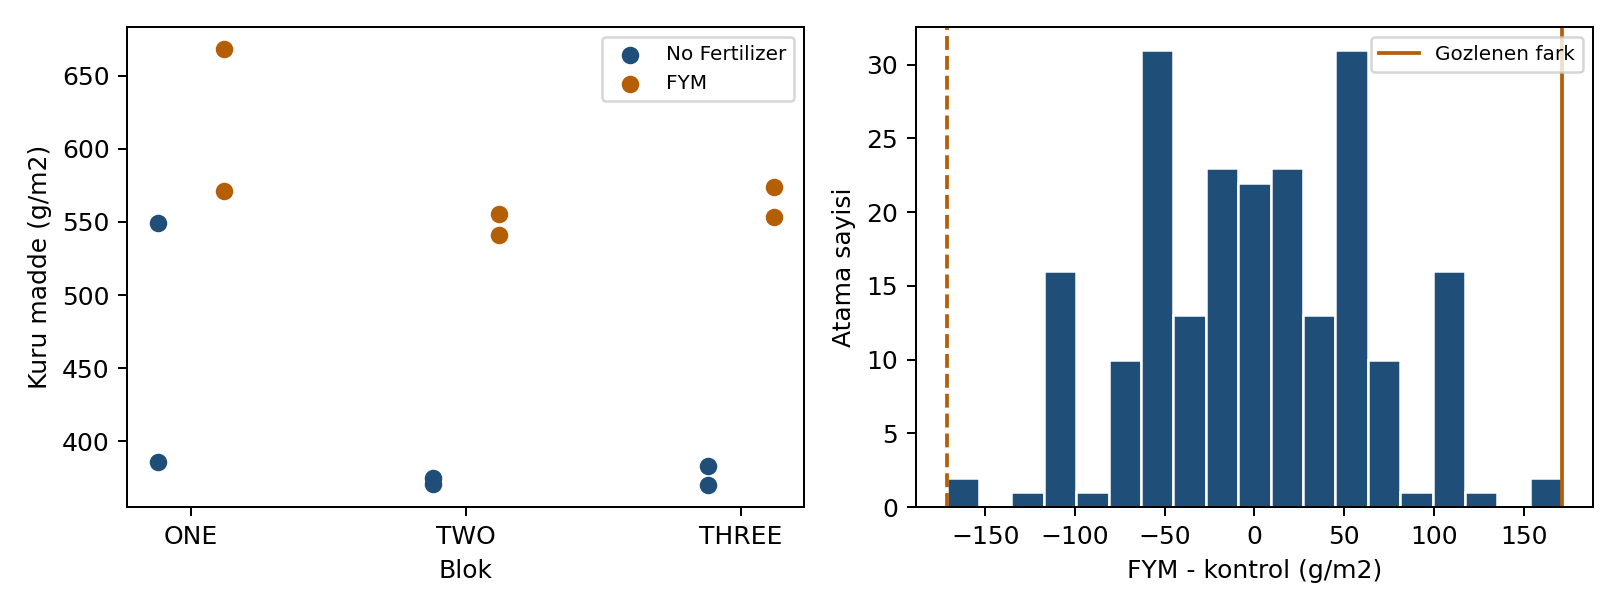
\includegraphics[width=\linewidth]{companion/vakalar/v1-colt-park/comparison.png}
\caption{Colt Park öğretim uyarlaması: solda 12 parselin yanıtı, sağda
216 koşullu atamanın fark dağılımı. Çizgiler gözlenen farkı ve negatifini
gösterir; histogram güven aralığı değildir.}
\label{fig:v1-colt-park}
\end{figure}

\textbf{Kontrol görevi.} Fark yönünü ters çevirin: tahminin işareti
değişmeli, mutlak değere dayalı iki yönlü $p$ aynı kalmalıdır.
Histogramın sınıf sayısını değiştirmenin tam sayım sonucunu neden
değiştirmediğini açıklayın; test grafiğin sütunlarından değil 216 değerden
hesaplanır.

\begin{assumptionbox}
Bootstrap, gözlenen örneklemin hedef evren için küçük bir temsil modeli gibi
kullanılmasına dayanır. Kolayda örnekleme, kapsam hatası, güçlü bağımlılık veya
çok küçük örneklem bu yaklaşımı zayıflatabilir. Kümeli, zaman serili ya da
eşleştirilmiş verilerde sıradan satır bootstrap'i yerine veri yapısını koruyan
yeniden örnekleme yöntemleri gerekir.
\end{assumptionbox}

\begin{mistakebox}
10.000 bootstrap tekrarı 10.000 yeni gözlem anlamına gelmez. Gerçek bilgi
miktarını özgün örneklem ve veri toplama tasarımı belirler. Tekrar sayısını
artırmak örnekleme yanlılığını veya yetersiz örneklem hacmini gidermez.
\end{mistakebox}

\begin{outputguidebox}
Yazılım çıktısında özgün tahmini, yeniden örnekleme tekrar sayısını, kullanılan
tohumu ve yeniden örnekleme birimini kontrol edin. Bootstrap çıktısında
standart hata ile aralık yöntemini; rastgeleleştirme çıktısında test
istatistiğini, yönü, uç tekrar sayısını ve \pval-değeri düzeltmesini birlikte
okuyun.
\end{outputguidebox}

\section{Çözümlü problemler}

\subsection*{Problem 1: Bütün bootstrap örneklemlerini oluşturma}

$2$ ve $6$ değerlerinden oluşan bir örneklemden, yerine koyarak iki gözlem
seçilsin. Olası bootstrap örneklemlerini ve ortalamalarını yazın; bootstrap
ortalamasının merkezini ve standart hatasını bulun.

\textbf{Çözüm.} Dört sıralı bootstrap örneklemi
\[
(2,2),\quad(2,6),\quad(6,2),\quad(6,6)
\]
ve ortalamaları sırasıyla $2,4,4,6$'dır. Dağılımın merkezi
\[
\bar\theta^*=\frac{2+4+4+6}{4}=4
\]
olup özgün örneklem ortalamasına eşittir. Dört eşit olasılıklı değerin
dağılım standart sapması
\[
\sqrt{\frac{(2-4)^2+(4-4)^2+(4-4)^2+(6-4)^2}{4}}
=\sqrt2\approx1{,}41
\]
olur. Bu küçük örnek bütün olası bootstrap sonuçlarını göstermek içindir;
uygulamada çok daha büyük örneklem ve tekrar sayıları kullanılır.

\subsection*{Problem 2: Bootstrap çıktısını yorumlama}

Bir ortalama tahmini 72,4, bootstrap standart hatası 1,8 ve yüzde 95 yüzdelik
aralığı $[68{,}9;75{,}8]$ bulunmuştur. Sonucu doğru biçimde yorumlayın.

\textbf{Çözüm.} Tahmin edilen evren ortalaması 72,4'tür. Bootstrap standart
hatası, aynı veri üretme sürecinde ortalama tahmininin örneklemden örnekleme
yaklaşık değişkenliğini 1,8 puan olarak özetler. Yüzdelik aralık, bootstrap
tekrar tahminlerinin orta yüzde 95'ini temel alarak parametre için 68,9 ile
75,8 arasındaki değerleri makul göstermektedir.

``Parametrenin bu aralıkta bulunma olasılığı yüzde 95'tir'' denmemelidir.
Ayrıca aralığın geçerliliği örneklemin temsil gücüne ve bootstrap şemasının
veri yapısına uygunluğuna bağlıdır.

\subsection*{Problem 3: Tekrar sayısı ve örneklem hacmi}

Bir araştırmacı $n=20$ gözlemden 1.000 bootstrap tekrarı üretmiş, daha sonra
tekrar sayısını 50.000'e çıkarmıştır. Hangi belirsizlik azalır, hangisi
değişmez?

\textbf{Çözüm.} Tekrar sayısının artması bootstrap standart hatası ve yüzdelik
noktalarının benzetimden kaynaklanan Monte Carlo dalgalanmasını azaltır.
Ancak özgün örneklem hâlâ 20 gözlemden oluşmaktadır. Veri setinin temsil
gücü, aykırı gözlemlere duyarlılığı ve küçük örneklemden kaynaklanan temel
belirsizliği değişmez. Yeni bilgi için yeniden örnekleme tekrarından değil,
uygun tasarımla toplanmış yeni bağımsız gözlemlerden yararlanmak gerekir.

\subsection*{Problem 4: Küçük bir kesin rastgeleleştirme testi}

A grubunun sonuçları $8,9$, B grubunun sonuçları $4,5$ olsun. İki kişilik A
grubu korunarak dört değerin bütün olası grup atamalarını değerlendirin.
Gözlenen ortalama farkı ve iki yönlü kesin \pval-değerini bulun.

\textbf{Çözüm.} Gözlenen fark
\[
T_{\text{göz}}=\frac{8+9}{2}-\frac{4+5}{2}=4
\]
olur. Dört kişiden ikisini A grubuna seçmenin altı yolu vardır. Olası farklar
$4,-1,0,0,1,-4$ değerleridir. Mutlak değeri gözlenen $4$ kadar veya daha büyük
iki sonuç vardır. Bu nedenle iki yönlü kesin \pval-değeri
\[
p=\frac{2}{6}=0{,}333
\]
olur. Gözlenen fark büyük görünse de dört birimlik örneklem çok az olası
atama üretmektedir; sıfır hipotezini reddetmek için yeterli kanıt yoktur.

\subsection*{Problem 5: Monte Carlo \pval-değeri}

999 rastgeleleştirme tekrarının 18'inde gözlenen kadar veya daha uç bir test
istatistiği elde edilmiştir. Düzeltilmiş \pval-değerini hesaplayın.

\textbf{Çözüm.}
\[
p=\frac{18+1}{999+1}=\frac{19}{1000}=0{,}019.
\]
Sonuç yüzde 5 düzeyinde sıfır hipotezine karşı kanıt sunar. \pval-değerini
$18/999$ olarak hesaplamak sayısal olarak yakın olsa da artı bir düzeltmesi,
sonlu benzetimde sıfır \pval-değeri elde edilmesini ve gözlenen düzenlemenin
referans dağılımı dışında bırakılmasını önler.

\subsection*{Problem 6: Uygun yeniden örnekleme şemasını seçme}

Üç durumda uygun işlemi belirleyin: (a) bağımsız iki grubun ortalama farkı
için güven aralığı, (b) rastgele atanmış iki grubun farkı için sıfır hipotezi
testi, (c) aynı kişilerin ön test--son test farkı için sıfır değişim testi.

\textbf{Çözüm.} İlk durumda her grubun gözlemleri kendi grubu içinde yerine
koyarak seçilir ve ortalama farkı bootstrap ile tekrar hesaplanır. İkinci
durumda sonuçlar sabit tutularak grup etiketleri, özgün grup hacimleri
korunacak biçimde karıştırılır. Üçüncü durumda kişiler birbirinden bağımsız
birimler olarak korunur; her kişinin fark işareti sıfır hipotezi altında
rastgele çevrilir.

Bütün satırları tek bir havuzdan sıradan biçimde seçmek bu üç tasarımın
tamamında doğru değildir. Yeniden örnekleme, bağımsızlık ve eşleşme yapısını
korumalıdır.

\section{R ile çözümlü uygulama}
\label{sec:r-bootstrap}

\textbf{Soru.} Dış veri dosyası gerektirmeyen iki öğretim örneği kullanın:
$2,3,3,4,13$ değerlerinin ortalaması için bootstrap standart hatası ve
aralığı; $7,8,9$ ile $2,3,4$ grupları için tam permütasyon testi hesaplayın.
Bunlar bölümdeki gerçek veri analizlerinin yerine geçen yeni bulgular değildir.

\begin{lstlisting}[style=prismR]
set.seed(2026)
degerler <- c(2, 3, 3, 4, 13)
tekrar <- 10000
bootstrap <- replicate(tekrar,
  mean(sample(degerler, length(degerler), replace = TRUE)))
c(ortalama = mean(degerler), bootstrap_se = sd(bootstrap))
quantile(bootstrap, c(0.025, 0.975), type = 7)
sqrt(mean((degerler - mean(degerler))^2) / length(degerler))
tam_bootstrap <- expand.grid(rep(list(degerler), length(degerler)))
quantile(rowMeans(tam_bootstrap), c(0.025, 0.975), type = 7)
grup_a <- c(7, 8, 9)
grup_b <- c(2, 3, 4)
birlesik <- c(grup_a, grup_b)
gozlenen <- mean(grup_a) - mean(grup_b)
atamalar <- combn(seq_along(birlesik), length(grup_a))
farklar <- apply(atamalar, 2, function(indis) {
  mean(birlesik[indis]) - mean(birlesik[-indis])
})
p_tam <- mean(abs(farklar) >= abs(gozlenen) - 1e-12)
c(fark = gozlenen, atama_sayisi = ncol(atamalar), p = p_tam)
\end{lstlisting}

\begin{outputguidebox}
\textbf{Çözüm ve kontrol değerleri.} İlk örneğin ortalaması 5'tir.
Benzetimle bulunan bootstrap standart hatası, ampirik dağılım altında
hesaplanan 1,8111'e yaklaşır. Bütün $5^5=3125$ geri koymalı sıralı
örneklem listelenirse tam bootstrap yüzdelik aralığı $[2{,}6;9{,}0]$ olur;
10.000 tekrarlı benzetimin uçları küçük farklılıklar gösterebilir.
İkinci örnekte gözlenen fark $8-3=5$'tir. Olası $\binom{6}{3}=20$
atamanın ikisi mutlak değerce en az bu kadar uçtur; tam iki yönlü $p=0{,}10$ olur.
\end{outputguidebox}

\textbf{Yorum.} Bootstrap geri koymalı, grup etiketlerinin permütasyonu
geri koymasızdır. Yalnız beş gözlem ve belirgin bir uç değer içeren ilk örnek,
güvenilir kapsama garantisi değil yöntem gösterimidir. Tam sayımda
\texttt{+1} düzeltmesi uygulanmaz; bu düzeltme sınırlı rastgele permütasyonla
yaklaştırılan testler içindir. Permütasyon testi uygun etiket değiştirilebilirliği
veya bu atamaları üreten rastgele atama tasarımını gerektirir.

\textbf{Pekiştirme ve yanıt.} Gözlenen fark büyük görünse de bu çok küçük
örnekte çift yönlü $p=0{,}10$ olduğundan yüzde 5 düzeyinde $H_0$ reddedilemez.
Bu sonuç iki evrenin aynı olduğunun kanıtı değildir.

\begin{etkinlik}
Yeniden örnekleme planınızı denetleyin: Analiz birimi korunuyor mu? Yeniden
örneklenen şey gözlem, küme, eş veya etiket mi? Üretilen dağılım tahmin
belirsizliğini mi yoksa sıfır hipotezini mi temsil ediyor?
\end{etkinlik}

\section{Bölüm özeti}

\begin{itemize}
  \item Bootstrap, gözlemleri yerine koyarak seçip tahminin değişkenliğini yaklaşıklar.
  \item Bootstrap standart hatası tekrar tahminlerinin standart sapmasıdır.
  \item Yüzdelik aralık tekrar dağılımının alt ve üst yüzdeliklerine dayanır.
  \item Rastgeleleştirme testi sıfır hipotezi altında etiket veya işaretleri değiştirir.
  \item Tekrar sayısı Monte Carlo hatasını azaltır; özgün örneklem hacmini büyütmez.
  \item Yeniden örnekleme şeması analiz birimini, kümeleri ve eşleşmeleri korumalıdır.
\end{itemize}

\bolumkaynaklari{\cite{efron1993,davison1997,good2005}}

\section*{Alıştırmalar}

\begin{enumerate}
  \item Bootstrap örneklemesinde neden yerine koyarak seçim yapıldığını açıklayın.
  \item Bootstrap dağılımı ile kuramsal örnekleme dağılımını karşılaştırın.
  \item $B$ tekrar sayısını artırmanın etkisini örneklem hacmini artırmaktan ayırın.
  \item $3,7$ örnekleminden hacmi iki olan bütün bootstrap örneklemlerini yazın.
  \item Bootstrap tekrarlarının standart sapmasının hangi niceliği tahmin ettiğini belirtin.
  \item Yüzde 90 yüzdelik bootstrap aralığında kullanılacak yüzdelikleri yazın.
  \item Bootstrap'in seçim yanlılığını neden gideremediğini açıklayın.
  \item İki bağımsız grup için etiket karıştırma işlemini adım adım yazın.
  \item 4.999 tekrarın 124'ünde uç sonuç elde edilirse düzeltilmiş \pval-değerini hesaplayın.
  \item İki yönlü ve üst yönlü rastgeleleştirme \pval-değerlerinin uçluk tanımlarını karşılaştırın.
  \item Eşleştirilmiş veride grup etiketlerini bağımsızmış gibi karıştırmanın sakıncasını açıklayın.
  \item Kümeli okul verisi için sıradan satır bootstrap'inin neden uygun olmayabileceğini tartışın.
  \item Bootstrap aralığının güçlü çarpıklıkta hangi nedenle başarısız olabileceğini açıklayın.
  \item Gerçek veri uygulamasında 0,405 oran farkı ile $p=0{,}0267$ sonucunu etki büyüklüğü ve nedensellik bakımından yorumlayın.
  \item Aynı veri üzerinde bootstrap ve rastgeleleştirme yöntemlerinin yanıtladığı soruları karşılaştırın.
  \item Yeniden üretilebilir bir benzetim raporunda verilmesi gereken en az beş bilgiyi yazın.
\end{enumerate}

\bolumbaglantisi{chapters/09-bootstrap-rastgelelestirme.tex}